\documentclass[t]{beamer}
%\documentclass[finnish,english,handout]{beamer}

% Uncomment if want to show notes
% \setbeameroption{show notes}

\mode<presentation>
{
  \usetheme{Copenhagen}
  % oder ...
  
  %\setbeamercovered{transparent}
  % oder auch nicht
}


\usepackage[T1]{fontenc}
\usepackage[latin1]{inputenc}
\usepackage{times}
\usepackage{epic,epsfig}
\usepackage{subfigure,float}
\usepackage{amsmath,amsfonts,amssymb}
\usepackage{inputenc}
\usepackage{afterpage}
\usepackage{url}
\urlstyle{same}
\usepackage{amsbsy}
\usepackage{eucal}
\usepackage{rotating}
\usepackage{listings}
\usepackage{lstbayes}
\usepackage[all,poly,ps,color]{xy}
\usepackage{eurosym}
\usepackage{microtype}

\usepackage{natbib}
\bibliographystyle{apalike}

\hypersetup{%
  bookmarksopen=true,
  bookmarksnumbered=true,
  pdftitle={Stan},
  pdfsubject={Bayesian data analysis},
  pdfauthor={Aki Vehtari},
  pdfkeywords={},
  pdfstartview={FitH -32768},
  colorlinks=true,
  linkcolor=navyblue,
  citecolor=navyblue,
  filecolor=navyblue,
  urlcolor=navyblue
}

% \definecolor{hutblue}{rgb}{0,0.2549,0.6784}
% \definecolor{midnightblue}{rgb}{0.0977,0.0977,0.4375}
% \definecolor{hutsilver}{rgb}{0.4863,0.4784,0.4784}
% \definecolor{lightgray}{rgb}{0.95,0.95,0.95}
% \definecolor{section}{rgb}{0,0.2549,0.6784}
% \definecolor{list1}{rgb}{0,0.2549,0.6784}
\definecolor{forestgreen}{rgb}{0.1333,0.5451,0.1333}
\definecolor{navyblue}{rgb}{0,0,0.5}
\renewcommand{\emph}[1]{\textcolor{navyblue}{#1}}

\graphicspath{{./figs/}}

\pdfinfo{            
  /Title      (Bayesian data analysis 4)
  /Author     (Aki Vehtari) % 
  /Keywords   (Bayesian probability theory, Bayesian inference, Bayesian data analysis)
}


\parindent=0pt
\parskip=8pt
\tolerance=9000
\abovedisplayshortskip=0pt

\setbeamertemplate{navigation symbols}{}
\setbeamertemplate{headline}[default]{}
\setbeamertemplate{headline}[text line]{\insertsection}
\setbeamertemplate{footline}[frame number]


\def\o{{\mathbf o}}
\def\t{{\mathbf \theta}}
\def\w{{\mathbf w}}
\def\x{{\mathbf x}}
\def\y{{\mathbf y}}
\def\z{{\mathbf z}}

\DeclareMathOperator{\E}{E}
\DeclareMathOperator{\Var}{Var}
\DeclareMathOperator{\var}{var}
\DeclareMathOperator{\Sd}{Sd}
\DeclareMathOperator{\sd}{sd}
\DeclareMathOperator{\Gammad}{Gamma}
\DeclareMathOperator{\Invgamma}{Inv-gamma}
\DeclareMathOperator{\Bin}{Bin}
\DeclareMathOperator{\Negbin}{Neg-bin}
\DeclareMathOperator{\Poisson}{Poisson}
\DeclareMathOperator{\Beta}{Beta}
\DeclareMathOperator{\logit}{logit}
\DeclareMathOperator{\N}{N}
\DeclareMathOperator{\U}{U}
\DeclareMathOperator{\BF}{BF}
\DeclareMathOperator{\Invchi2}{Inv-\chi^2}
\DeclareMathOperator{\NInvchi2}{N-Inv-\chi^2}
\DeclareMathOperator{\InvWishart}{Inv-Wishart}
\DeclareMathOperator{\tr}{tr}
% \DeclareMathOperator{\Pr}{Pr}
\def\euro{{\footnotesize \EUR\, }}
\DeclareMathOperator{\rep}{\mathrm{rep}}



\title[]{Bayesian data analysis}
\subtitle{}

\author{Aki Vehtari}

\institute[Aalto]{}


\begin{document} 

\begin{frame}

  {\Large\color{navyblue} Chapter 4}

  \begin{itemize}
  \item 4.1 Normal approximation (Laplace's method)
  \item 4.2 Large-sample theory
  \item 4.3 Counter examples
    \begin{itemize}
    \item includes examples of difficult posteriors for MCMC, too
    \end{itemize}
  \item 4.4 Frequency evaluation*
  \item 4.5 Other statistical methods*
  \end{itemize}

\end{frame}

\begin{frame}

    {\Large\color{navyblue} Normal approximation (Laplace approximation)}

  \begin{itemize}
  \item Often posterior converges to normal distribution when
    $n\rightarrow \infty$
  \item If posterior is unimodal and close to symmetric
    \begin{itemize}
    \item we can approximate $p(\theta|y)$ with normal distribution
    \begin{align*}
      p(\theta|y)&\approx \frac{1}{\sqrt{2\pi}\sigma_\theta}\exp\left(-\frac{1}{2\sigma_\theta^2}(\theta-\hat{\theta})^2\right)
    \end{align*}
  \item<2-3> Laplace used this (before Gauss) to approximate the
    posterior of binomial model to infer ratio of girls and boys born
  \item<3> A most strict proof by LeCam in 1950's
  \end{itemize}
\end{itemize}
\vspace{-2.5\baselineskip}
    \uncover<4->{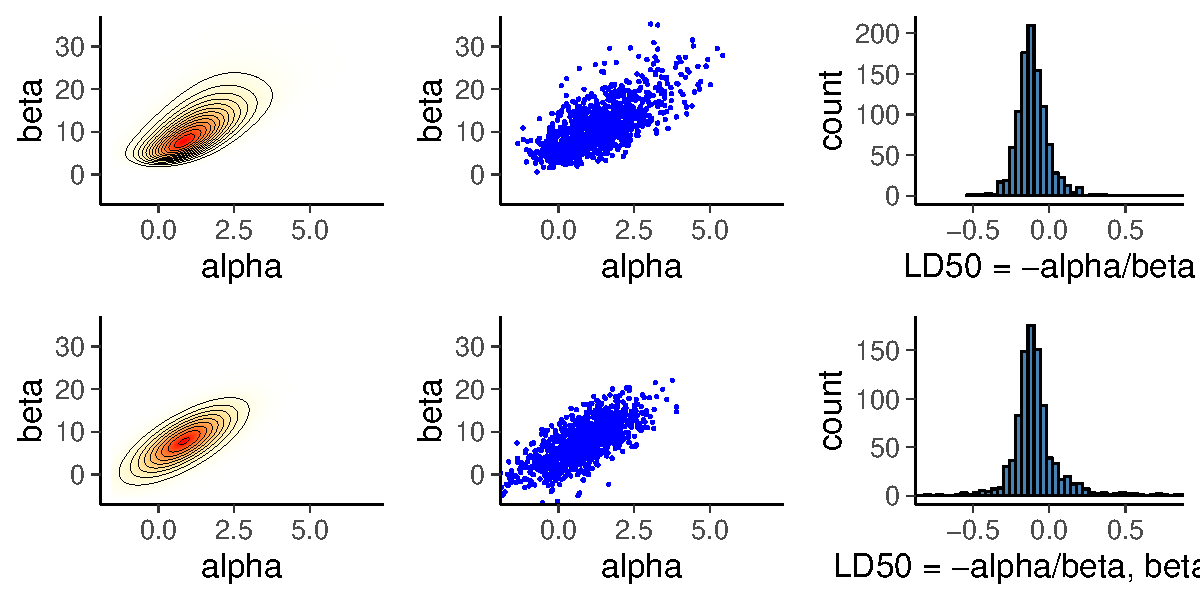
\includegraphics[width=10cm]{bioassay_norm.pdf}}

\end{frame}

\begin{frame}

    {\Large\color{navyblue} Taylor series}
  
  \begin{itemize}
    \item We can approximate $p(\theta|y)$ with normal distribution
    \begin{align*}
      p(\theta|y)&\approx \frac{1}{\sqrt{2\pi}\sigma_\theta}\exp\left(-\frac{1}{2\sigma_\theta^2}(\theta-\hat{\theta})^2\right)
    \end{align*}
      \begin{itemize}
      \item i.e. log posterior $\log p(\theta|y)$ can be
        approximated with a quadratic function
      \end{itemize}
    \begin{align*}
      \log p(\theta|y)& \approx \alpha(\theta-\hat{\theta})^2 + C
    \end{align*}
  \item<2-> Univariate Taylor series expansion around $\theta=\hat{\theta}$
    \begin{equation*}
      f(\theta)=f(\hat{\theta}) {\only<3->{\color{gray}}+ f'(\hat{\theta})(\theta-\hat{\theta})} + \frac{f''(\hat{\theta})}{2!}(\theta-\hat{\theta})^2 {\only<4->{\color{gray}} +\frac{f^{(3)}(\hat{\theta})}{3!}(\theta-\hat{\theta})^3+\ldots}
    \end{equation*}
    \begin{itemize}
    \item<3-> if $\hat{\theta}$ is at mode, then $f'(\hat{\theta})=0$
    \item<4-> often when $n \rightarrow \infty$, $\frac{f^{(3)}(\hat{\theta})}{3!}(\theta-\hat{\theta})^3+\ldots$ is small
    \end{itemize}
  \end{itemize}
  
\end{frame}

\begin{frame}

    {\Large\color{navyblue} Multivariate Taylor series}
  
  \begin{itemize}
    \item Multivariate series expansion
      \begin{equation*}
        f(\theta)= f(\hat{\theta}) {\color{gray} + \frac{d f(\theta')}{d \theta'}_{\theta'=\hat{\theta}}(\theta-\hat{\theta})}
        + \frac{1}{2!}(\theta-\hat{\theta})^T  \frac{d^2 f(\theta')}{d \theta'^2}_{\theta'=\hat{\theta}} (\theta-\hat{\theta}) {\color{gray} + \ldots}
          % \sum_{j=0}^\infty\left\{\frac{1}{j!}\left[\sum_{k=1}^n(x_k-a_k)\frac{\partial}{\partial x_k'}\right]^j
          % f(x_1',\ldots,x_n')\right\}_{x_1'=a_1,\ldots,x_n'=a_n}
      \end{equation*}~
  \end{itemize}
  
\end{frame}

% \note{Onko joku joka ei muista Taylorin sarjakehitelm��?
% Nimetty 1700-luvulla el�nnen Taylorin mukaan

%PIIRTELE TAULULLE}

\begin{frame}

    {\Large\color{navyblue} Normal approximation}

    \begin{itemize}
      \only<1-2>{
  \item Taylor series expansion of the log posterior around the posterior mode
    $\hat{\theta}$
    \begin{equation*}
      \log p(\theta|y) = \log p(\hat{\theta}|y) +
      \frac{1}{2}(\theta-\hat{\theta})^T\left[\frac{d^2}{d\theta^2}\log p(\theta'|y) \right]_{\theta'=\hat{\theta}} (\theta-\hat{\theta})+\ldots
    \end{equation*}
    }
  \item<2-> Multivariate normal $\propto\left|\Sigma\right|^{-1/2} \exp\left(-\frac{1}{2}(\theta-\hat{\theta}^T)\Sigma^{-1}(\theta-\hat{\theta})\right)$
  \end{itemize}
  \vspace{-0.5\baselineskip}
  \only<3>{
    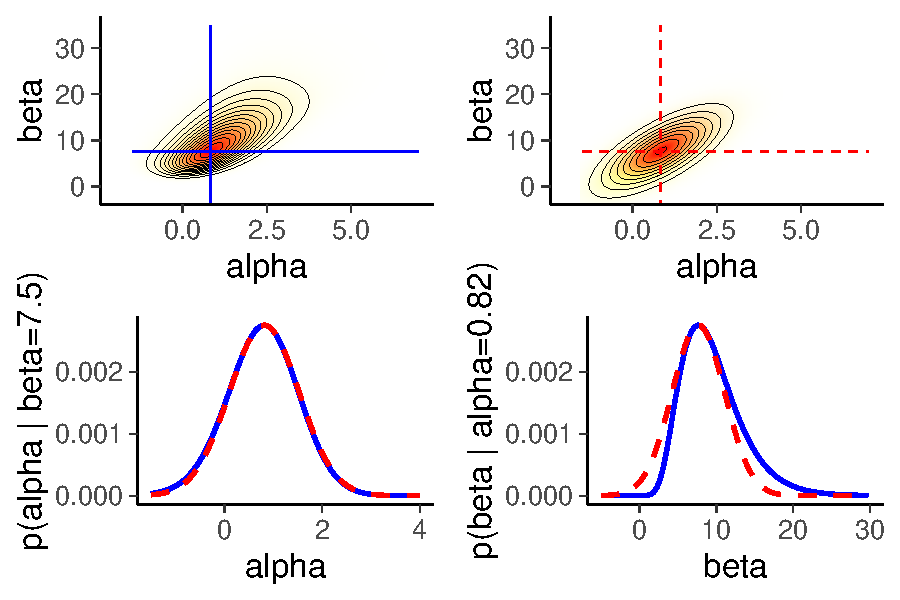
\includegraphics[width=11cm]{cond_excat_norm.pdf}}
  \only<4>{
    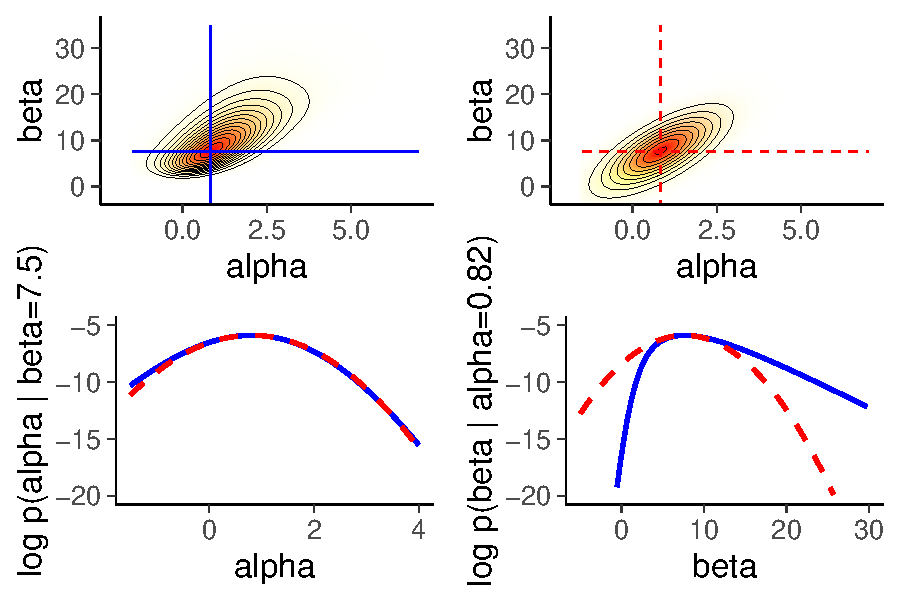
\includegraphics[width=11cm]{cond_excat_norm_log.pdf}}

\end{frame}

\begin{frame}

    {\Large\color{navyblue} Normal approximation}

  \begin{itemize}
  \item Taylor series expansion of the log posterior around the posterior mode
    $\hat{\theta}$
    \begin{equation*}
      \log p(\theta|y) = \log p(\hat{\theta}|y) +
      \frac{1}{2}(\theta-\hat{\theta})^T\left[\frac{d^2}{d\theta^2}\log p(\theta'|y) \right]_{\theta'=\hat{\theta}} (\theta-\hat{\theta})+\ldots
    \end{equation*}
  \item Multivariate normal $\propto\left|\Sigma\right|^{-1/2} \exp\left(-\frac{1}{2}(\theta-\hat{\theta}^T)\Sigma^{-1}(\theta-\hat{\theta})\right)$

  \item Normal approximation 
    \begin{equation*}
      p(\theta|y) \approx \N(\hat{\theta},[I(\hat{\theta})]^{-1})
    \end{equation*}
    where $I(\theta)$ is called {\em observed information}
    \begin{equation*}
      I(\theta) = - \frac{d^2}{d\theta^2}\log p(\theta|y)
    \end{equation*}
  \end{itemize}

\end{frame}

\begin{frame}

    {\Large\color{navyblue} Normal approximation}

  \begin{itemize}
  \item $I(\theta)$ is called {\em observed information}
    \begin{equation*}
      I(\theta) = - \frac{d^2}{d\theta^2}\log p(\theta|y)
    \end{equation*}
    \begin{itemize}
    \item $I(\hat{\theta})$ is the second derivatives at the mode and
      thus describes the curvature at the mode
    \item if the mode is inside the parameter space, $I(\hat{\theta})$
      is positive
    \item if $\theta$ is a vector, then $I(\theta)$ is a matrix
%    \item K�ytet��n my�s nimityst� {\em Hessian} $H(\theta)$
  \end{itemize}
\end{itemize}

\end{frame}

\begin{frame}

    {\Large\color{navyblue} Normal approximation}

    \begin{itemize}
    \item BDA3 Ch 4 has an example where it is easy to compute first
      and second derivatives and there is easy analytic solution to
      find where the first derivatives are zero
    \end{itemize}
    
\end{frame}
  
\begin{frame}

    {\Large\color{navyblue} Normal approximation -- example}

  \begin{itemize}
    \item Normal distribution, unknown mean and variance
      \begin{itemize}
        \item uniform prior $(\mu,\log\sigma)$
        \item normal approximation for the posterior of $(\mu,\log\sigma)$
      \end{itemize}
      \begin{eqnarray*}
        \log
        p(\mu,\log\sigma|y)=& \mathrm{constant}-n\log\sigma- \\
        & \frac{1}{2\sigma^2}[(n-1)s^2 + n(\bar{y}-\mu)^2]
      \end{eqnarray*}
      \pause
      first derivatives
      \begin{eqnarray*}
        \frac{d}{d\mu}\log p(\mu,\log\sigma|y) & = & \frac{n(\bar{y}-\mu)}{\sigma^2},\\
        \pause
        \frac{d}{d(\log\sigma)}\log p(\mu,\log\sigma|y) &
         = &  -n + \frac{(n-1)s^2+n(\bar{y}-\mu)^2}{\sigma^2},
      \end{eqnarray*}
      \pause
      from which it is easy to compute the mode
      \begin{eqnarray*}
        (\hat{\mu},\log\hat{\sigma})=\left(\bar{y},\frac{1}{2}\log\left(\frac{n-1}{n}s^2\right)\right)
      \end{eqnarray*}
  \end{itemize}

\end{frame}

% \note{t�ss� parametrisoidaan malli $\log\sigma$:n avulla\\
% muistanette varmaankin, ett� priorina uniformi priori $\log\sigma$:lle
% vastaa $1/\sigma$ prioria sigmalle, joka voidaan
% muuttujanvaihdoksella helposti todeta

% \begin{align*}
%   p(\log\sigma)&=|J|p(\sigma)=\frac{d \sigma}{d\log\sigma} \frac{1}{\sigma}=\sigma \frac{1}{\sigma}=1
% \end{align*}

% \begin{align*}
%   \frac{d}{d\mu}(\bar{y}-\mu)^2=-2(\bar{y}-\mu)
% \end{align*}

% \begin{align*}
%   \frac{d}{d\log\sigma}\sigma^{-2}=\frac{d}{d\log\sigma}\exp(\log\sigma)^{-2}=-2\exp(\log\sigma)^{-3}(\log\sigma)=-2\exp(\log\sigma)^{-2}=-2 \sigma^{-2}
% \end{align*}
%  % LASKE muuttujanvaihdos valmiiksi!
% }

\begin{frame}

    {\Large\color{navyblue} Normal approximation -- example}

  \begin{itemize}
    \item Normal distribution, unknown mean and variance\\
      first derivatives
      \begin{eqnarray*}
        \frac{d}{d\mu}\log p(\mu,\log\sigma|y) & = & \frac{n(\bar{y}-\mu)}{\sigma^2},\\
        \frac{d}{d(\log\sigma)}\log p(\mu,\log\sigma|y) & = & -n + \frac{(n-1)s^2+n(\bar{y}-\mu)^2}{\sigma^2}
      \end{eqnarray*}
      \pause
      second derivatives
      \begin{eqnarray*}
        \frac{d^2}{d\mu^2}\log p(\mu,\log\sigma|y) & = & -\frac{n}{\sigma^2},\\
        \pause \frac{d^2}{d\mu d(\log\sigma)}\log p(\mu,\log\sigma|y) & 
        = & -2n\frac{\bar{y}-\mu}{\sigma^2},\\
        \pause \frac{d^2}{d(\log\sigma)^2}\log p(\mu,\log\sigma|y) & 
        = & -\frac{2}{\sigma^2}((n-1)s^2+n(\bar{y}-\mu)^2)
      \end{eqnarray*}
  \end{itemize}

\end{frame}

\begin{frame}

    {\Large\color{navyblue} Normal approximation -- example}

  \begin{itemize}
    \item Normal distribution, unknown mean and variance\\
      second derivatives
      \begin{eqnarray*}
        \frac{d^2}{d\mu^2}\log p(\mu,\log\sigma|y) & = & -\frac{n}{\sigma^2},\\
        \frac{d^2}{d\mu(\log\sigma)}\log p(\mu,\log\sigma|y) & = & -2n\frac{\bar{y}-\mu}{\sigma^2},\\
        \frac{d^2}{d(\log\sigma)^2}\log p(\mu,\log\sigma|y) & = & -\frac{2}{\sigma^2}((n-1)s^2+n(\bar{y}-\mu)^2)
      \end{eqnarray*}
      matrix of the second derivatives at $(\hat{\mu},\log\hat{\sigma})$
      \begin{eqnarray*}
        \begin{pmatrix}
          -n/\hat{\sigma}^2 & 0 \\
          0 & -2n
        \end{pmatrix}
      \end{eqnarray*}
  \end{itemize}

\end{frame}

\begin{frame}

    {\Large\color{navyblue} Normal approximation -- example}

  \begin{itemize}
    \item Normal distribution, unknown mean and variance\\
      posterior mode
      \begin{eqnarray*}
        (\hat{\mu},\log\hat{\sigma})=\left(\bar{y},\frac{1}{2}\log\left(\frac{n-1}{n}s^2\right)\right)
      \end{eqnarray*}
      matrix of the second derivatives at $(\hat{\mu},\log\hat{\sigma})$
      \begin{eqnarray*}
        \begin{pmatrix}
          -n/\hat{\sigma}^2 & 0 \\
          0 & -2n
        \end{pmatrix}
      \end{eqnarray*}
      normal approximation
      \begin{equation*}
        p(\mu,\log\sigma|y) \approx \N\left(
          \begin{pmatrix}
            \mu \\ \log\sigma
          \end{pmatrix}
          \Bigg|
          \begin{pmatrix}
            \bar{y} \\ \log\hat{\sigma}
          \end{pmatrix},
        \begin{pmatrix}
          \hat{\sigma}^2/n & 0 \\
          0 & 1/(2n)
        \end{pmatrix}
        \right)
      \end{equation*}
  \end{itemize}

\end{frame}

\begin{frame}[fragile]

    {\Large\color{navyblue} Normal approximation -- numerically}

  \begin{itemize}
  \item Normal approximation can be computed numerically
    \begin{itemize}
    \item iterative optimization to find a mode (maye use gradients)
    \item autodiff or finite-difference for gradients and Hessian
    \item<2> e.g. in R, demo4\_1.R:
    {\scriptsize
\begin{lstlisting}[language=R]
bioassayfun <- function(w, df) {
  z <- w[1] + w[2]*df$x
  -sum(df$y*(z) - df$n*log1p(exp(z)))
}

theta0 <- c(0,0)
optimres <- optim(w0, bioassayfun, gr=NULL, df1, hessian=T)
thetahat <- optimres$par
Sigma <- solve(optimres$hessian)
\end{lstlisting}
      }
    \end{itemize}
  \end{itemize}
\end{frame}

\begin{frame}[fragile]

    {\Large\color{navyblue} Normal approximation -- numerically}

  \begin{itemize}
  \item Normal approximation can be computed numerically
    \begin{itemize}
    \item iterative optimization to find a mode (maye use gradients)
    \item autodiff or finite-difference for gradients and Hessian
    \end{itemize}
  \item RStanARM has an option {\small\tt algorithm='optimizing'}
    \uncover<2->{
    \begin{itemize}
    \item uses L-BFGS quasi-Newton optimization algorithm for finding the mode
    \item uses autodiff for gradients
    \item uses finite differences of gradients to compute Hessian
      \begin{itemize}
      \item<3-> second order autodiff coming to Stan 
      \end{itemize}
    \end{itemize}
    }
  \end{itemize}
\end{frame}

\begin{frame}

    {\Large\color{navyblue} Normal approximation}

  \begin{itemize}
  \item Optimization and computation of Hessian requires usually much
    less density evaluations than MCMC
  \item<2-> In some cases accuracy is sufficient
  \item<3-> In some cases accuracy for a conditional distribution is
    sufficient (Ch 13)
    \begin{itemize}
    \item e.g. Gaussian latent variable models, such as Gaussian
      processes (Ch 21)
      \begin{itemize}
      \item CS-E4070 - Special Course in Machine Learning and Data
        Science: Gaussian processes - theory and applications
    \end{itemize}
    \end{itemize}
  \item<4-> Accuracy can be improved by importance sampling (Ch 10)
  \end{itemize}
\end{frame}

\begin{frame}
  
  {\Large\color{navyblue} Example: Importance sampling in Bioassay}

   \vspace{-.5\baselineskip}
   \makebox[12cm][t]{
     \hspace{-0.9cm}
     \begin{minipage}[t][12cm][t]{12cm}
       \begin{center}
        \makebox[0cm][t]{\hspace{-0.5cm}\rotatebox{90}{\hspace{1cm}Grid}}
        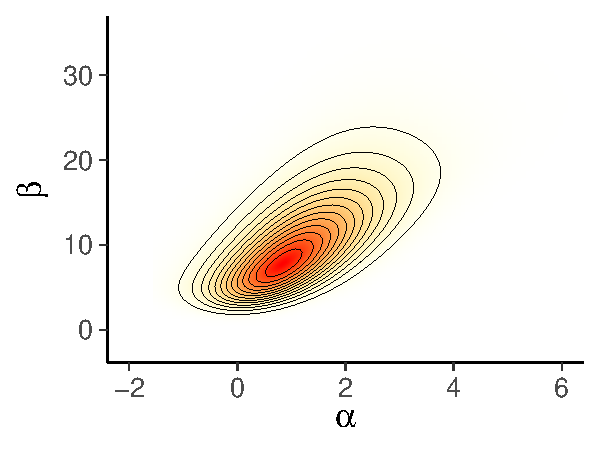
\includegraphics[width=3.4cm]{bioassayis1d.pdf}
      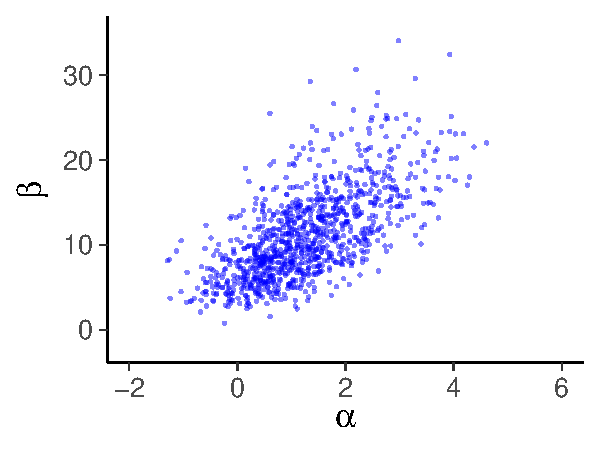
\includegraphics[width=3.4cm]{bioassayis1s.pdf}
      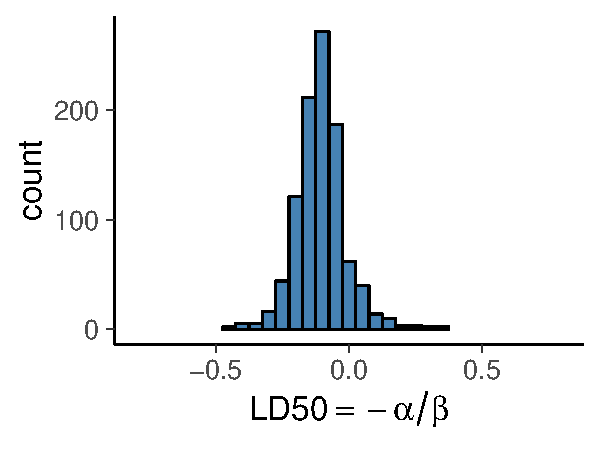
\includegraphics[width=3.4cm]{bioassayis1h.pdf}\\
      \only<2->{
        \makebox[0cm][t]{\hspace{-0.5cm}\rotatebox{90}{\hspace{1cm}Normal}}
      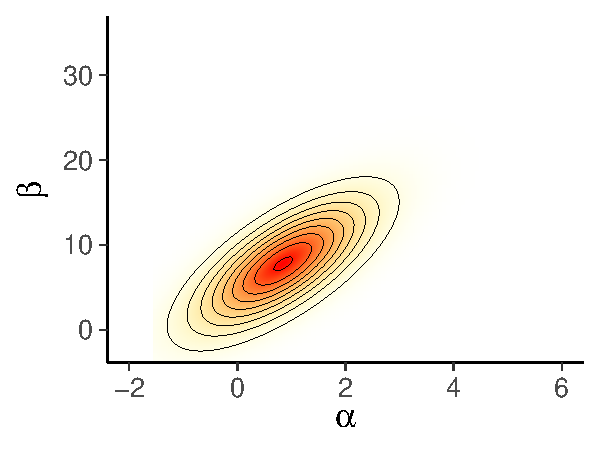
\includegraphics[width=3.4cm]{bioassayis2d.pdf}
      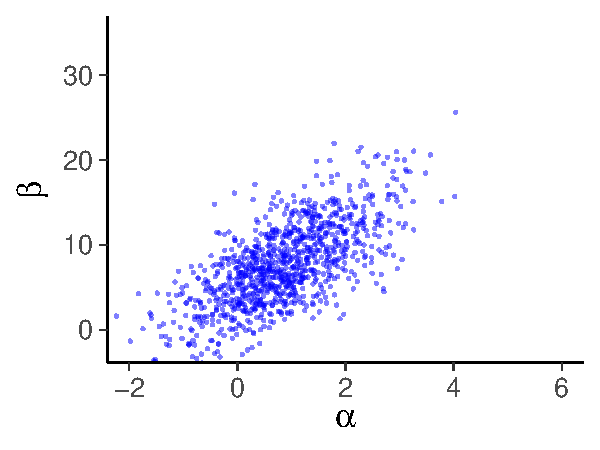
\includegraphics[width=3.4cm]{bioassayis2s.pdf}
      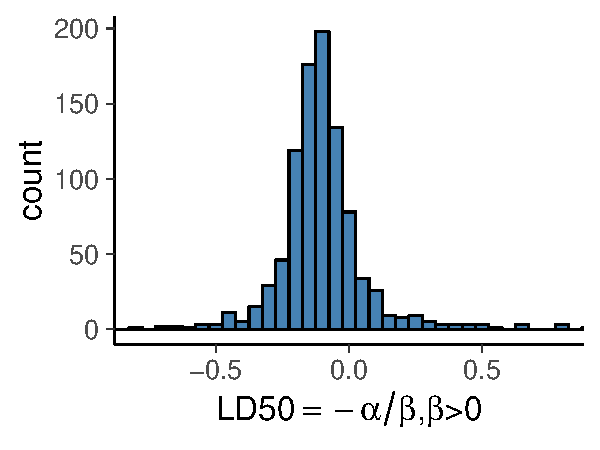
\includegraphics[width=3.4cm]{bioassayis2h.pdf}\\}
    \only<2-3>{Normal approximation is discussed more in BDA3 Ch 4\\}
    \only<3>{But the normal approximation is not that good here:\\ Grid sd(LD50) $\approx$ 0.1, Normal sd(LD50) $\approx$ .75!}
      \only<4->{
        \makebox[0cm][t]{\hspace{-0.5cm}\rotatebox{90}{\hspace{1cm}SIR}}
      
\includegraphics[width=3.4cm]{bioassayis3d.pdf}
      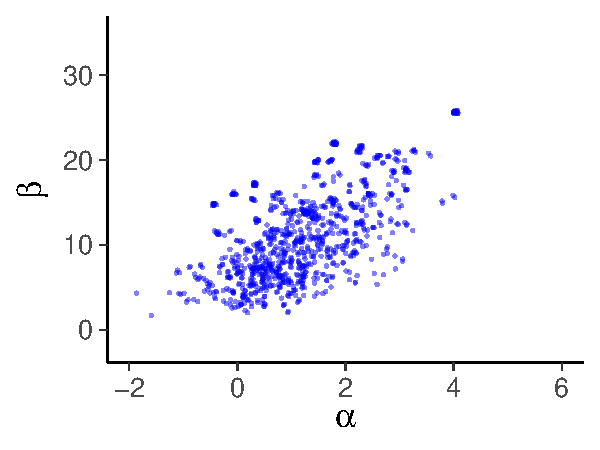
\includegraphics[width=3.4cm]{bioassayis3s.pdf}
      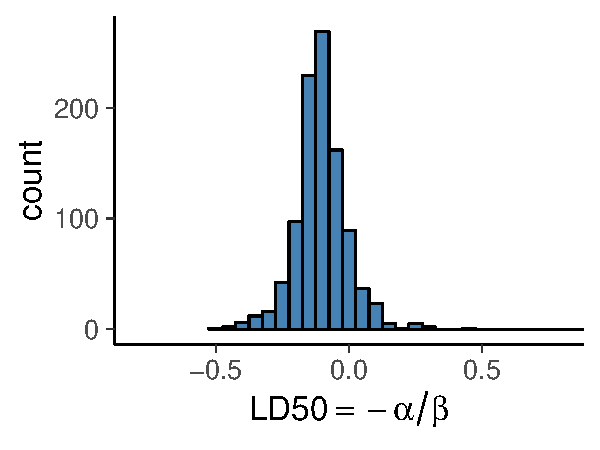
\includegraphics[width=3.4cm]{bioassayis3h.pdf}\\}
    \only<5->{Grid sd(LD50) $\approx$ 0.1, SIR sd(LD50) $\approx$ 0.1}
    \end{center}
     \end{minipage}  
   }
  
\end{frame}

\begin{frame}

    {\Large\color{navyblue} Normal approximation}

  \begin{itemize}
  \item Accuracy can be improved by importance sampling
  \item Pareto-$k$ diagnostic of importance sampling weights can be
    used for diagnostic
    \begin{itemize}
    \item in Bioassay example $k=0.57$, which is ok
    \end{itemize}
  \end{itemize}
\end{frame}


\begin{frame}

    {\Large\color{navyblue} Other distributional approximations*}

    \begin{itemize}
    \item<+-> Higher order derivatives at the mode can be used
    \item<+-> Split-normal and split-$t$ by Geweke use additional
      scaling along different principal axes
    \item<+-> Other distributions can be used
    \item<+-> Instead of mode and Hessian at mode, e.g.
      \begin{itemize}
      \item variational inference (Ch 13)
        \begin{itemize}
        \item CS-E4820 - Machine Learning: Advanced Probabilistic Methods
        \item Stan has an experimental ADVI algorithm
        \end{itemize}
      \item expectation propagation  (Ch 13)
      \item speed of these is usually between optimization and MCMC
      \end{itemize}
    \end{itemize}

\end{frame}

\begin{frame}

    {\Large\color{navyblue} Distributional approximations}

    \vspace{-.25\baselineskip}
{\small {\color{blue} Exact}, {\color{red} Normal at mode}, {\color{forestgreen} Normal with variational inference}}
    
  \makebox[12cm][t]{
    \hspace{-.7cm}
\begin{minipage}[t]{12cm}
  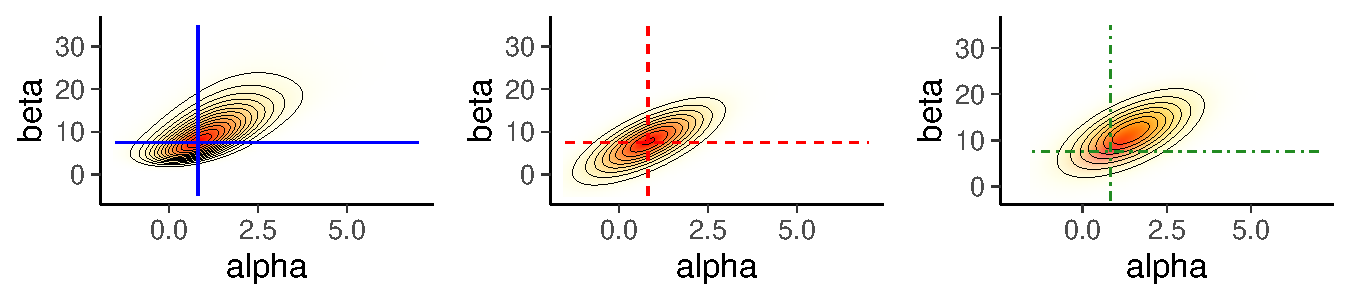
\includegraphics[width=12cm]{cond_excat_normfr2.pdf}\\
   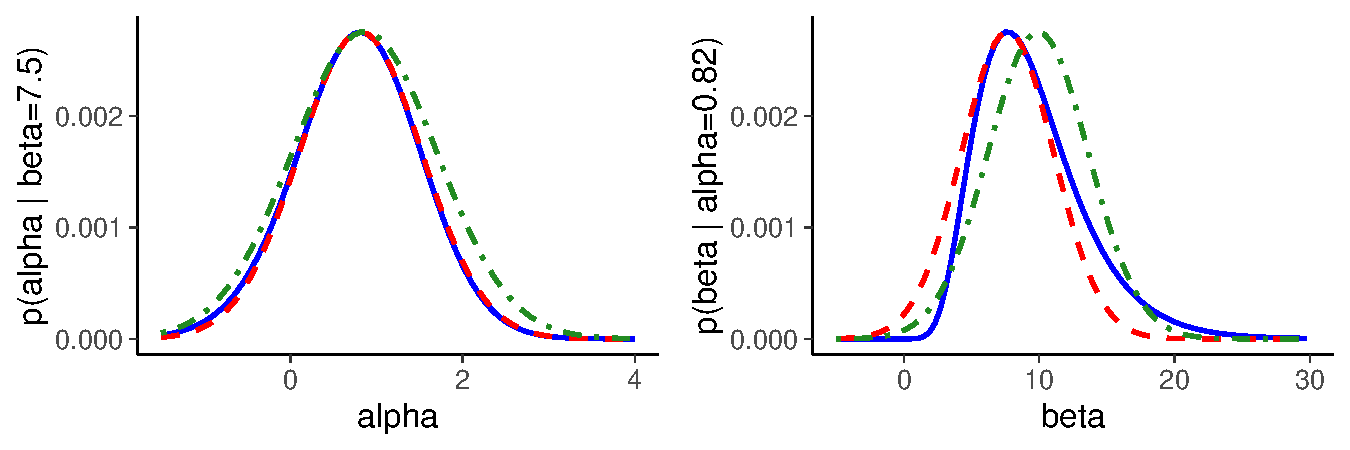
\includegraphics[width=12cm]{cond_excat_normfr3.pdf}
 \end{minipage}
}

    \vspace{-.5\baselineskip}
\uncover<2->{\footnotesize
  Grid sd(LD50) $\approx$ 0.090,\\
  Normal sd(LD50) $\approx$ .75,
  Normal + SIR sd(LD50) $\approx$ 0.096 (Pareto-$k$ = 0.57)\\}
\uncover<3->{\footnotesize
  VI sd(LD50) $\approx$ 0.13,
  VI + SIR sd(LD50) $\approx$ 0.095 (Pareto-$k$ = 0.17)
  }

\end{frame}

\begin{frame}

    {\Large\color{navyblue} Large sample theory}
  
  \begin{itemize}
  \item Asymptotic normality
    \begin{itemize}
    \item<+-> as $n$ the number of observations $y_i$ increases the
      posterior converges to normal distribution
    \item<+-> can be shown by showing that
      \begin{itemize}
      \item eventually likelihood dominates the prior
      \item the higher order terms in Taylor series increase slower
        than the second order term
      \end{itemize}
    \item<+-> see counter examples
    \end{itemize}
\end{itemize}
\end{frame}

\begin{frame}

    {\Large\color{navyblue} Large sample theory}
  
  \begin{itemize}
  \item Assume "true" underlying data distribution $f(y)$
    \begin{itemize}
    \item observations $y_1,\ldots,y_n$ are independent samples from
      the joint distribution $f(y)$
    \item "true" data distribution $f(y)$ is not always well defined
    \item in the following we proceed as if there were true underlying data distribution
    \item for the theory the exact form of $f(y)$ is not important as
      long at it has certain regularity conditions
    \end{itemize}
  \end{itemize}

\end{frame}

\begin{frame}

    {\Large\color{navyblue} Large sample theory}
  
  \begin{itemize}
  % \item Asymptoottinen normaalius
  %   \begin{itemize}
  %   \item jakaumasta $f(y)$ saatujen havaintojen $y_i$ m��r�n $n$ kasvaessa
  %     parametrivektorin posteriorijakauma l�hestyy normaalijakaumaa
  %   \end{itemize}
  %   \pause
  \item Consistency
    \begin{itemize}
    \item if true distribution is included in the parametric family,
      so that $f(y)=p(y|\theta_0)$ for some $\theta_0$, then posterior
      converges to a point $\theta_0$, when $n\rightarrow\infty$
    \item<2-> a point doesn't have uncertainty 
    \item<3-> same result as for maximum likelihood estimate
    \end{itemize}
  \item<4-> If true distribution is not included in the parametric family,
    then there is no true $\theta_0$
    \begin{itemize}
    \item true $\theta_0$ is replaced with $\theta_0$ which minimizes
      the Kullback-Leibler divergence from $f(y)$
        \begin{align*}
          H(\theta_0)=\int f(y_i) \log\left(\frac{f(y_i)}{p(y_i|\theta_0)}\right)dy_i
        \end{align*}
      \item<5-> this point doesn't have uncertainty, but it's a wrong point!
      \item<6-> same result as for maximum likelihood estimate
    \end{itemize}
\end{itemize}

\end{frame}

\begin{frame}

    {\Large\color{navyblue} Large sample theory -- counter examples}
  
  \begin{itemize}
    \item Under- and non-identifiability
      \begin{itemize}
      \item a model is under-identifiable, if the model has parameters or parameter combinations for which there is no information in the data
      \item then there is no single point $\theta_0$ where
        posterior would converge
      \item<2-> e.g. if the model is
        \begin{align*}
          y \sim \N(a+b+cx, \sigma)
        \end{align*}
        \begin{itemize}
          \vspace{-\baselineskip}
        \item<3-> posterior would converge to a line with prior
          determining the density along the line
        \end{itemize}
      \item<4-> e.g. if we never observe $u$ and $v$ at the same time and the model is
        \begin{equation*}
          \begin{pmatrix}
            u \\ v
          \end{pmatrix}
          \sim
          \N\left(
            \begin{pmatrix}
              0\\0
            \end{pmatrix},
            \begin{pmatrix}
              1 & \rho \\ \rho & 1
            \end{pmatrix}
            \right)
        \end{equation*}
        then correlation $\rho$ is non-identifiable
        \begin{itemize}
        \item<5-> e.g. $u$ and $v$ could be length and weight of
          a student; if only one of them is measured for each student,
          then $\rho$ is non-identifiable
      \end{itemize}
      \end{itemize}
      \item<6-> Problem also for other inference methods like MCMC
  \end{itemize}

\end{frame}

% \note{ongelma voidaan poistaa havaitsemalla ongelma, jos n�it�
% parametreja oikeasti tarvitsee estimoida hankitaan tarpeelliset havainnot}

\begin{frame}

    {\Large\color{navyblue} Large sample theory -- counter examples}
  
  \begin{itemize}
    % \item Does not always hold when $n\rightarrow\infty$
    \item If the number of parameter increases as the number of
      observation increases
      \begin{itemize}
      \item in some models number of parameters depends on the number
        of observations
        \item e.g. time series models $y_i \sim
          \N(\theta_i,\sigma^2)$ and $\theta_i$ has prior in time
        \item posterior of $\theta_i$ does not converge to a point, if
          additional observations do not bring enough information
      \end{itemize}
  \end{itemize}

\end{frame}

\begin{frame}

    {\Large\color{navyblue} Large sample theory -- counter examples}
  
  \begin{itemize}
    % \item Does not always hold when $n\rightarrow\infty$
    \item Aliasing (FI: \emph{valetoisto})
      \begin{itemize}
      \item special case of under-identifiability where likelihood
        repeats in separate points
      \item e.g. mixture of normals
        \begin{equation*}
          p(y_i|\mu_1,\mu_2,\sigma_1^2,\sigma_2^2,\lambda)=\lambda\N(\mu_1,\sigma_1^2)+(1-\lambda)\N(\mu_2,\sigma_2^2)
        \end{equation*}
        \uncover<2->{
        if $(\mu_1,\mu_2)$ are switched, $(\sigma_1^2,\sigma_2^2)$ are
        switched and replace $\lambda$ with $(1-\lambda)$, model is
        equivalent; posterior would usually have two modes which are
        mirror images of each other and the posterior does not
        converge to a single point}
    \end{itemize}
  \item<3-> For MCMC makes the convergence diagnostics more difficult,
    as it is difficult to identify aliasing from other multimodality
\end{itemize}

\end{frame}

\begin{frame}

    {\Large\color{navyblue} Large sample theory -- counter examples}
  
  \begin{itemize}
    % \item Does not always hold when $n\rightarrow\infty$
    \item Unbounded (FI: \emph{rajoittamaton}) likelihood
      \begin{itemize}
      \item if likelihood is unbounded it is possible that there is no
        mode in the posterior
      \item<2-> e.g. previous normal mixture model; assume $\lambda$ to be
        known (and not $0$ or $1$); if we set $\mu_1=y_i$ for any $i$
        and $\sigma_1^2\rightarrow 0$, then likelihood
        $\rightarrow\infty$
      \item<3-> if prior for $\sigma_1^2$ does not go to zero when
        $\sigma_1^2\rightarrow 0$, then the posterior is unbounded
      \item<4-> when $n\rightarrow\infty$ the number of likelihood
        modes increases
      \end{itemize}
    \item<5-> Problem for any inference method including MCMC
      \begin{itemize}
      \item can be avoided with good priors
      \item<6-> note that a prior close to a prior allowing unbounded
        posterior may produce almost unbounded posterior
      \end{itemize}
  \end{itemize}

\end{frame}

% \note{esim. uniformi priori ei hyv�

% esim. $1/\sigma^2$ priori ei hyv�

% esim. $\Invchi2$-jakauma sopivilla parametreilla mahdollinen}

\begin{frame}

    {\Large\color{navyblue} Large sample theory -- counter examples}
  
  \begin{itemize}
    % \item Does not always hold when $n\rightarrow\infty$
  \item Improper posterior
    \begin{itemize}
    \item asymptotic results assume that probability sums to 1
    \item e.g. Binomial model, with $\Beta(0,0)$ prior and observation $y=n$
      \begin{itemize}
      \item posterior $p(\theta|n,0)=\theta^{n-1}(1-\theta)^{-1}$
      \item when $\theta\rightarrow 1$, then
        $p(\theta|n,0)\rightarrow \infty$
      \end{itemize}
    \end{itemize}
  \item<2-> Problem for any inference method including MCMC
    \begin{itemize}
    \item can be avoided with proper priors
    \item<3-> note that prior close to a improper prior may produce
      almost improper posterior
    \end{itemize}
  \end{itemize}

\end{frame}

% \note{my�s sellainen ei-aito priori k�y, joka tuottaa aidon posteriorin

% Muistakaa, ett� $\Beta(1,1)$ vastaa uniformiprioria ja
% $\Beta(\frac{1}{2},\frac{1}{2})$ Jeffereysin prioria, joten
% $\Beta(0,0)$ on viel� v�ljempi priori ja onkin ei-aito

% posteriori $\Beta(\theta|n,0)=\theta^{n-1}(1-\theta)-1$\\
% $\Beta(1|n,0)=1^{n-1}0^{-1} = 1/0 = \infty$
% }

\begin{frame}

    {\Large\color{navyblue} Large sample theory -- counter examples}
  
  \begin{itemize}
    % \item Does not always hold when $n\rightarrow\infty$
    \item Prior distribution does not include the convergence point
      \begin{itemize}
      \item if in discrete case $p(\theta_0)=0$ or in continuous case
        $p(\theta)=0$ in the neighborhood of $\theta_0$, then the
        convergence results based on the dominance of the likelihood
        do not hold 
      \end{itemize}
    \item<2-> Should have a positive prior probability/density where needed
\end{itemize}

\end{frame}

\begin{frame}

    {\Large\color{navyblue} Large sample theory -- counter examples}
  
  \begin{itemize}
    % \item Does not always hold when $n\rightarrow\infty$
    \item Convergence point at the edge of the parameter space
      \begin{itemize}
      \item if $\theta_0$ is on the edge of the parameter space,
        Taylor series expansion has to be truncated, and normal
        approximation does not necessarily hold
        \item<2-> e.g. $y_i\sim\N(\theta,1)$ with a restriction $\theta\geq
          0$ and assume that $\theta_0=0$
          \begin{itemize}
          \item posterior of $\theta$ is left truncated normal
            distribution with $\mu=\bar{y}$
        \item in the limit $n\rightarrow\infty$ posterior is half
          normal distribution \pause
        \end{itemize}
      \end{itemize}
    \item Can be easy or difficult for MCMC
  \end{itemize}

\end{frame}

\begin{frame}

    {\Large\color{navyblue} Large sample theory -- counter examples}
  
  \begin{itemize}
  \item Tails of the distribution
    \begin{itemize}
    \item normal approximation may be accurate for the most of the
      posterior mass, but still be inaccurate for the tails
    \item e.g. parameter which is constrained to be positive; given a
      finite $n$, normal approximation assumes non-zero probability
      for negative values
    \end{itemize}
  % \item Monte Carlo has different kind of problems with the tails
  \end{itemize}
  
\end{frame}


\begin{frame}

    {\Large\color{navyblue} Frequency evaluations}

    \begin{itemize}
    \item Bayesian theory has epistemic and aleatory probabilities
    \item Frequency evaluations focus on frequency properties given
      aleatoric repetition of an observation and modeling
      \begin{itemize}
      \item<2-> Consistency
      \item<3-> Asymptotic unbiasedness
        \begin{itemize}
        \item not that important in Bayesian inference
        \end{itemize}
      \item<4-> Asymptotic efficiency
        \begin{itemize}
        \item no other point estimate with smalle squared error
        \end{itemize}
      \item<5-> Calibration
        \begin{itemize}
        \item $\alpha\%$-posterior interval has the true value in
          $\alpha\%$ cases
        \item $\alpha\%$-predictive interval has the true future values
          in $\alpha\%$ cases
        \end{itemize}
      \end{itemize}
    \end{itemize}
    

\end{frame}

\end{document}

%%% Local Variables: 
%%% TeX-PDF-mode: t
%%% TeX-master: t
%%% End: 
